\section{Malware Attacks and Countermeasures}
\subsection{Malware attacks}
Malware attacks are common cyberattacks that exploit malicious software to execute unauthorized actions on the victim's system.\\
The burst of the internet contributed to a vast spread of various malware types. Among the most known types, there are:
\begin{itemize}
\item \textbf{Ransomware}, malware that threatens to publish the victim's personal data or block access to it unless a ransom is paid, encrypting data with malicious intent. Such attacks are usually carried out using a \textit{trojan} disguised as a legitimate file (for instance, an attachment to an email) and relying on the poor social engineering skills of the users. However, this is not always the case, as the \textit{WannaCry} ransomware proved, exploiting a vulnerability of the structure it spread across.\\
The user immediately detects a ransomware attack due to payment warnings that pop up.
\item \textbf{Spyware}, malware that is particularly hard to detect. It collects information about the victim's internet searches or even credit card data.\\
Email attachments or downloads from file-sharing platforms represent typical injection methods for such malware.\\
The victim usually experiences unusual behaviors of the system, such as new search engine tools.
\end{itemize}
\subsection{Malware Honeypots}

Defending yourself from malware attacks might not be trivial. Many people rely on antivirus software, that offers protection either for free or on a subscription.\\
Many antivirus firms rely on research honeypots to update their knowledge about the software that must be labeled as "dangerous" and create a \textit{malware signature} that can be stored in a database of known threats.\\
You can use malware honeypots to update such databases, they are supposed to act as a decoy for attackers. In some cases, they should also incentive the attacker to infect a system, to study the behavior of the malicious software. This is the case of high interaction honeypots, that can even simulate entire systems to be more appealing to attackers.\\
On the other hand, you can also just use malware honeypots to defend yourself from attackers.\\
Literature offers multiple ways you can design and deploy malware honeypots, ranging from simple to complex solutions. Some of the studies are listed below:
\begin{enumerate}
\item The usage of sentinel files in a network against ransomware;
\item The monitoring of changes in files within a short interval of time;
\item The usage of software diversification;
\item The usage of machine learning algorithms.
\end{enumerate}

\subsubsection{Sentinel Files}
A simple honeypot that intends to defend the system against ransomware, both the ones already known to the antivirus database and those not yet listed, could make use of sentinel files.\\
Such files act as \textit{trip wires} for the trap to be triggered. You keep the original hash digest of the sentinel files aside. Since ransomware tends to encrypt data, if an attack is in progress you will see more and more files changing content.
The strategy simply aims at monitoring changes in the digest of the sentinel files, to detect a ransomware attack and shutdown services before it spreads.\\
These files do not provide any production value and therefore every interaction with them (changes or removal) is to be considered malicious.\\
This is one of the few ways to deal with ransomware, since it is a particularly tough malware to defeat, it enters the victim's systems encrypted and so infection is nearly impossible to prevent.


\subsubsection{Frequent changes to files}
Some malware families aim at making the system busy by performing frequent changes to files within a short time. For small networks, you can monitor all file accesses and set a threshold above which you can state that probably a malware attack is in progress. \\
Heuristics can help since setting a low threshold might not allow authorized actions and a high threshold might not detect malware activities properly.\\
You can link thresholds of file changes to various degrees of response, as shown in the figure below.

\begin{figure}[ht!]
\centering
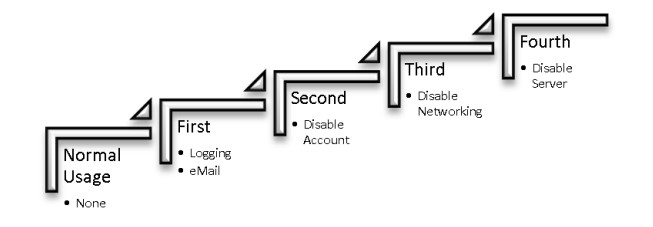
\includegraphics[width = 14cm]{images/responses.jpg}
\caption{ Gradual responses to file changes according to thresholds set by the admin.}
\label{fig:irradiances}
\end{figure}
\FloatBarrier

\noindent This mechanism allows you to set your response gradually, avoiding the shutdown of all services at once and therefore avoiding having a large recovery time once the system is restarted.\\
A proprietary solution called \textit{EventSentry} offers this file integrity monitoring service, letting the user deploy a honeypot that monitors files of interest via GUI.

\subsubsection{Software Diversification}
Studies prove that one of the keys to the success of malware attacks is that attackers rely on the so-called "software monoculture". In other words, it is much more likely that an attack is successful when the software implementation of the victim's system or infrastructure is easy to guess.\\
A \textit{system call} is the way for a computer program to interact with the kernel of the operating system on which it is executed.\\
Two sets of system calls (well-known ones and hidden ones) can detect attacks if you let the trusted nodes only use the hidden ones, which are less likely to be guessed. Any traffic on the network that relies on the interface of well-known system calls is to be considered malicious.\\
This solution allows you to let malware run freely and without any risk to the assets you want to defend. Thus, you can study the behavior of the malware and gather more information about it.\\
A drawback of this approach is that the malware attack could utilize the code already present in allowed operations.

%\subsubsection{Hybrid Honeypot: Low interaction + High interaction}
%\textcolor{red}{This honeypot framework got built for the IoT world, observing the vulnerabilities of IoT devices. It provides both a high interaction honeypot that simulates the services available in the system making them seem real and therefore very appealing for attackers and a low interaction honeypot with SSH service, to simulate the login procedure.}

\subsubsection{Machine Learning algorithms}
Literature is full of machine learning-based approaches regarding malware detection. They all use some kind of malware classifier whose purpose is to distinguish between malicious and benign software, with a certain degree of confidence. Here the system exposes some fake services and learns how to defend itself thanks to a training period that exploits a training data set, called "EMBER" as described in the article "The Endgame Malware BEnchmark for Research" \cite{https://doi.org/10.48550/arxiv.1804.04637}, which provides 900.000 training samples.\\
A classification technique often adopted in malware detection is the Decision Tree Algorithm, which classifies them based on malware features and behavior.\\
When malware is detected the honeypot gives some details to the admin, which is supposed to be a cybersecurity expert, who can validate or deny the classification, making the algorithm train even further.\\
As an example, ransomware always carries a message through which the user is warned that they should pay a ransom (often asked in untraceable currency, like bitcoins) to get their data back from the malicious encryption.
This feature could be exploited for defense purposes because as soon as a malicious text is spotted through keywords such as "pay", "blocked", etc you stop its spread.\\
This is just an example since ransomware might not carry this message, or it might be encrypted. A high training period with a wide training data set could help you spot malware by features (e.g., some peculiar file size and code fragments) rather than by a ransom message.

\begin{figure}[h]
\centering
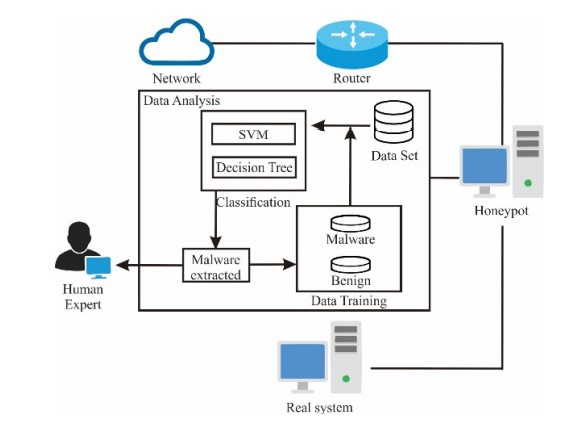
\includegraphics[width = 14cm]{images/machineLearning.jpg}
\caption{ Example architecture of system with honeypot and machine learning.}
\label{fig:irradiances}
\end{figure}
\FloatBarrier

\newpage

